\documentclass[pdftex,12pt,letter]{article}
\usepackage[binary-units=true]{siunitx}
\usepackage[margin=0.75in]{geometry}
\usepackage{verbatim}
\usepackage{graphicx}
\usepackage{cite}
\usepackage{color}
\usepackage[pdftex,pdfpagelabels,bookmarks,hyperindex,hyperfigures]{hyperref}
\usepackage{xspace}
\usepackage{amssymb}


\bibliographystyle{unsrt}

\newcommand{\fixme}[1]{\textbf{FIXME: #1}}    
\newcommand{\pd}{protoDUNE\xspace}
\newcommand{\singp}{Single Phase\xspace}
\newcommand{\dualp}{Dual Phase\xspace}


\title{The ProtoDUNE Experiments \\
Joint Data Challenge 2018}
\date{\today}
\author{TBA, C. Alt, N. Benekos, X. Espinal, S. Fuess, I. Furic, E. Pennacchio, R. Pordes,   \\
A. Norman, M. Potekhin, G. Savage, H. Schellman, S. Timm}

\begin{document}


\maketitle

\begin{abstract}

\noindent It is important to ensure 100\% readiness of the
end-to-end \pd software and computing complex during the detector commissioning period and
throughout data taking in 2018.  Following a \pd \singp  specific first data challenge in 2017 we propose a Joint ProtoDUNE  Data Challenge (known as DC2 or JDC) in order to identify
and address potential issues before they can impact the experiments.
This data challenge will include end-to-end testing of all components to be used for cosmic and beam data taking as far as they are available in the time frame. It is understood that these will not be final versions, especially as the data challenge aim is to find gaps and issues that could impact successful accomplishment of the experiments goals. 

The Joint Data Challenge is planned to take place the week of April 9th 2018.  We are using a mail list (dune-proto-joint-data-challenge@fnal.gov) and a DUNE SLACK channel (pd-datachallenges) for planning and technical details.  Documentation to be retained will be submitted to the DUNE DocDB. 
Working documents and results are being posted to the DUNE wiki:
\begin{verbatim}
https://wiki.dunescience.org/wiki/
ProtoDUNE_Dual_Phase_and_Single_Phase_Joint_Data_Challenge
\end{verbatim}
\end{abstract}

\tableofcontents

\pagebreak

\section{About this document}

The goal of this document is to provide the high level information and plan for  the Joint  \pd Data Challenge. The audience is the collaboration as a whole and  the  working groups contributing to the activities.
The document does not contain detailed descriptions
and/or designs of the computing
infrastructure elements and the reader is referred to existing documentation where
needed, with references provided in the text and references. 

\section{The Scope of the Joint Data Challenge}
This section will briefly describe the functional components, their scope and goals for the data challenge,  and any dependencies on other activities. During the planning stage we will aim to identify components that overlap and where software and functionalities might be shared and reused. 

Before any end-to-end data challenge can be meaningful, all individual components and interfaces must undergo
their own functional testing. The scope of the DC activity includes initial work on most of the components below and an
understanding of what files, file and data formats, and interfaces are going to be used. The evolving activities will be listed and tracked on the DUNE wiki. 

\subsection{Dual Phase Specifics}
\subsection{Single Phase Specifics}

\subsection{Assumptions about the software status and provisioning}
The Data Challenge will be done with the understanding that the software is not in its final state/readiness. It is assumed
however that the mechanism of software provisioning which leverage git and  CVMFS are in place and close to final.

\subsection{DAQ Online Buffer}
The DAQ Online Buffer which stores raw data assembled by the Event Builders, as files on disk. The internals
of the DAQ system itself are not within the scope of the DC, however the performance of the Online Buffer in the face of simultaneous data reading and writing will be tested. The DAQ Online Buffer will also be operated in two different modes - where simulated data files are provided and where data is being acquired in real time.

\subsection{Beam Instrumentation} 

\subsection{Slow Control Data}

\subsection{Online Monitoring System - do we actually need this component at this point?}
 
\subsection{Data Management}
The data management system is heavily used for data transport, archiving to tape at CERN and Fermilab, and access to the data in real time (including for data quality monitoring, remote archiving systems,  just in time processing and analysis at the CERN TIer-0, etc.). It includes the data cataloguing system (SAM).

The \textbf{Data Management System}\cite{docdb1212}  performs data transfers between a few endpoints
at CERN and FNAL starting with EOS (\dualp) and the Online Buffer (\singp), including output from DQM,  and which is also tasked with proper accounting and handling of the file catalog and other metadata
by interacting with the SAM system at FNAL (see next item). The Data Management/Handling System will also interface the disk-based mass storage
at CERN and FNAL (i.e.\,EOS\cite{eos} and dCache) as well as tape systems (CASTOR and Enstore respectively).
We anticipate using the \textit{Fermi File Transfer System} (also abbreviated as F-FTS\cite{fts}).

The \textbf{File Catalog (Metadata)}  -- SAM system at FNAL comprises the functionality of the file catalog, data storage and
retrieval based on Metadata and can also be used for orchestration of production workflows.

\subsection{Data Quality Monitoring (Single Phase only)}

In this Data Challenge, \textbf{Data Quality Monitoring} (DQM) will only be implemented for the Single Phase \pd.

The role of DQM is to run algorithms with turnaround time short enough to provide
actionable results  but which won't fit into the computational footprint of the Online Monitoring which is a part of the DAQ.
Typically DQM jobs are expected to run in under and hour and may involve workflows i.e. collections of jobs connected
by data and logic.

The DQM consists of the infrastructure part and the \textit{``payloads''} i.e. physics applications. 
The ProtoDUNE Prompt Processing System (\textbf{p3s}) \cite{docdb1811,p3s}  is the centerpiece
of the DQM infrastructure and is capable of running any type of DQM computations
as formulated and implemented by the detector experts. A dedicated Web
service will provide access to visual and data products coming out of DQM.

DC2 will include the most important physics workloads (payloads) as explicit components in the test.

\subsection{Keep Up Offline Reconstruction}

The Production Operations Management System is based on POMS. This FNAL-based service includes using the DUNE service portal, production workflows executed by POMS \cite{poms}, including the management and automation of  jobs
submission on distributed resources on the Grid. It will be the primary platform for \pd on which to run production and analysis.

\subsection{Offline Physics Processes}
\begin{itemize}
\item \textbf{Calibration}  TBD
 \item \textbf{Reconstruction}. While it is not expected that these components will be finalized
(and some even exist) at the time of the first Data Challenge it is important to have a firm grasp of the required interfaces,
data flow patterns and other crucial aspects of the \pd Reconstruction Systems.
\item \textbf{Data Reduction}.An optional (but desirable)  component of the overall \singp production chain is the Data Reduction step along the lines described
in \cite{docdb2089}.
\item \textbf{Analysis Suite Prototypes}. Same comment applies here as to the previous item, i.e.\,while there is no expectation
for the final design and implementation of the analysis chain to exist early in the experiment (especially that it is by nature the most
dynamic and fluid part of all software) it is important to put in place, document and optimize its interfaces with various components
of infrastructure e.g.\,calibration databases, Metadata, software and data provenance controls etc.
\end{itemize}


\subsection{Figures}
\noindent The relationship between the various infrastructure and other components listed above are schematically illustrated in
Fig.\ref{fig:dc2dp} and Fig.\ref{fig:dc1}. These diagram reflect the fact that transmission of \pd data is a multistage process and in particular there 
will be separate instances of some components operating across \dualp and \singp and in different  parts of the workflow processes. 
\begin{figure}[tbh]
  \centering
  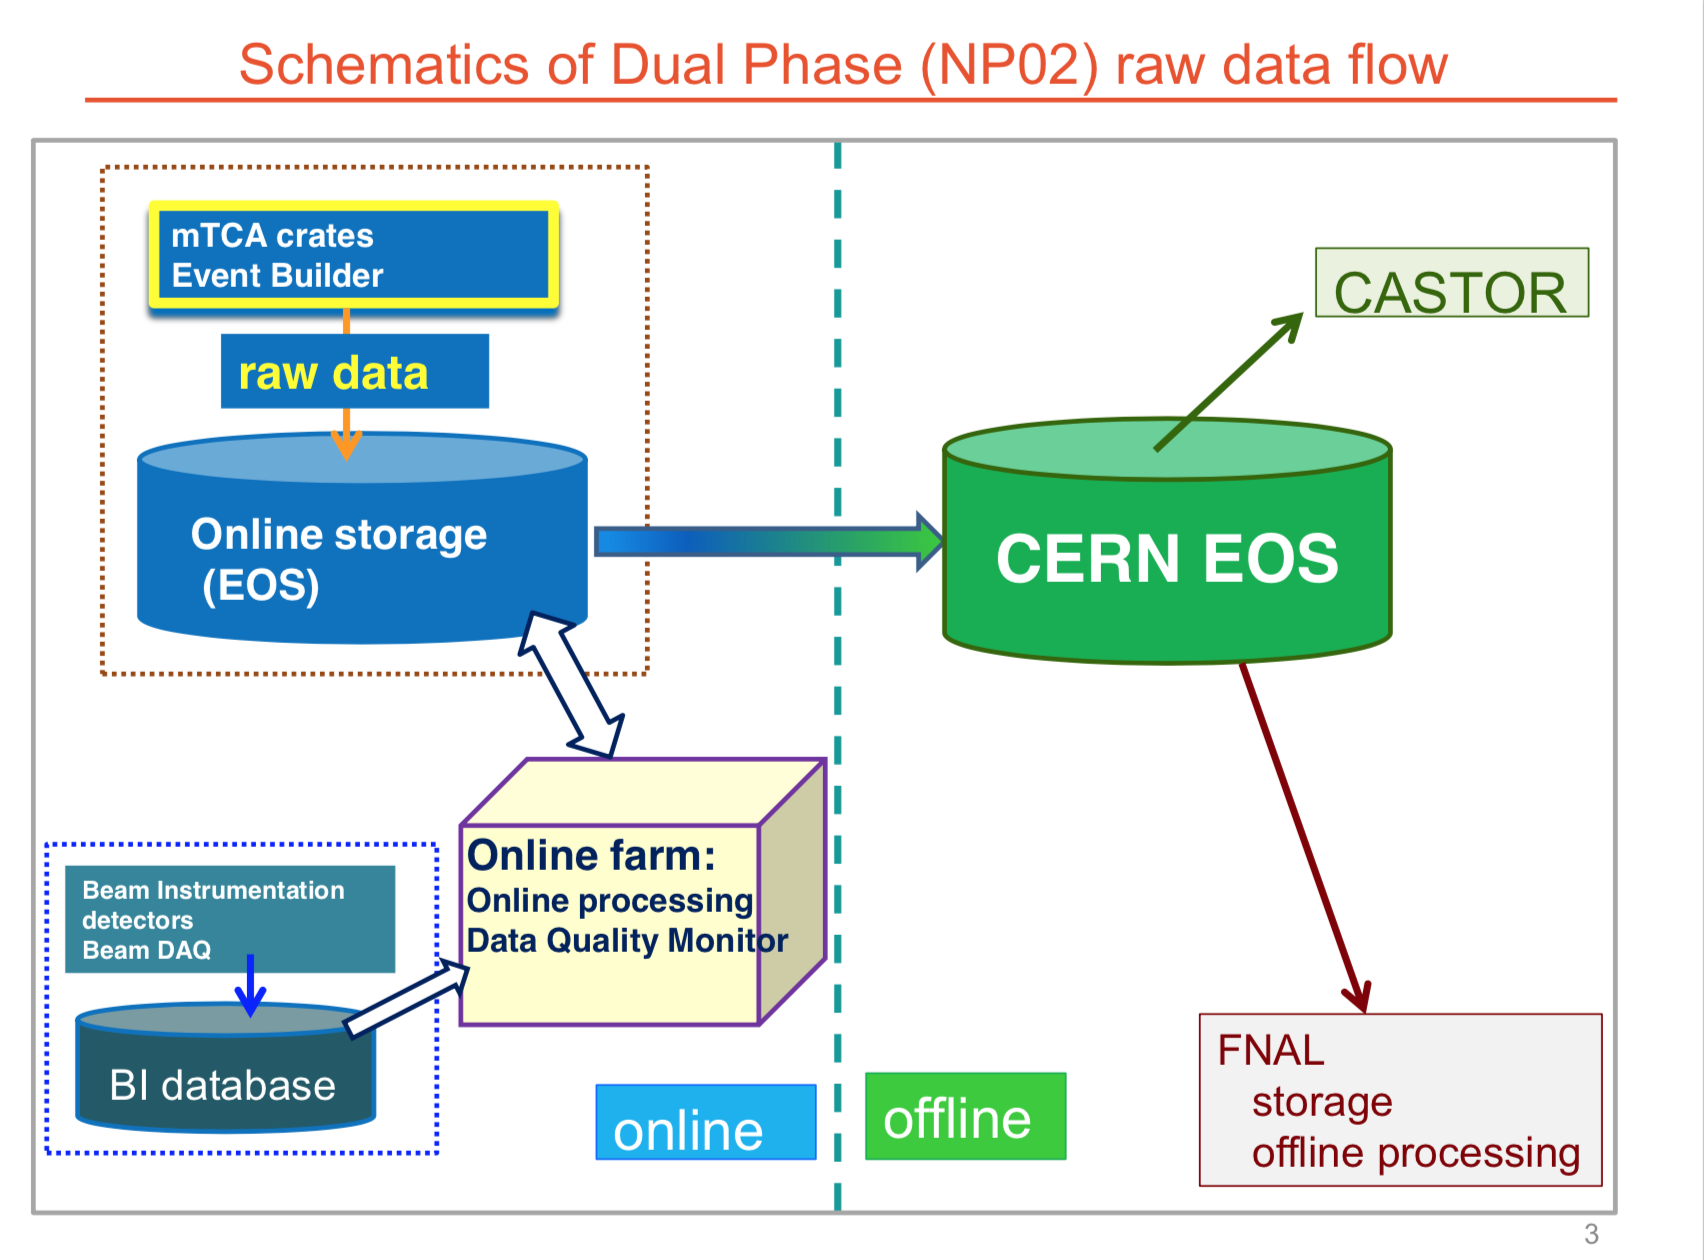
\includegraphics[width=1.0\textwidth]{../figures/DualPhaseDataFlow.png}
  \caption{Schematics of data flow and  processing in \pd \dualp data challenge.}
  \label{fig:dc2dp}
\end{figure}


\begin{figure}[tbh]
  \centering
  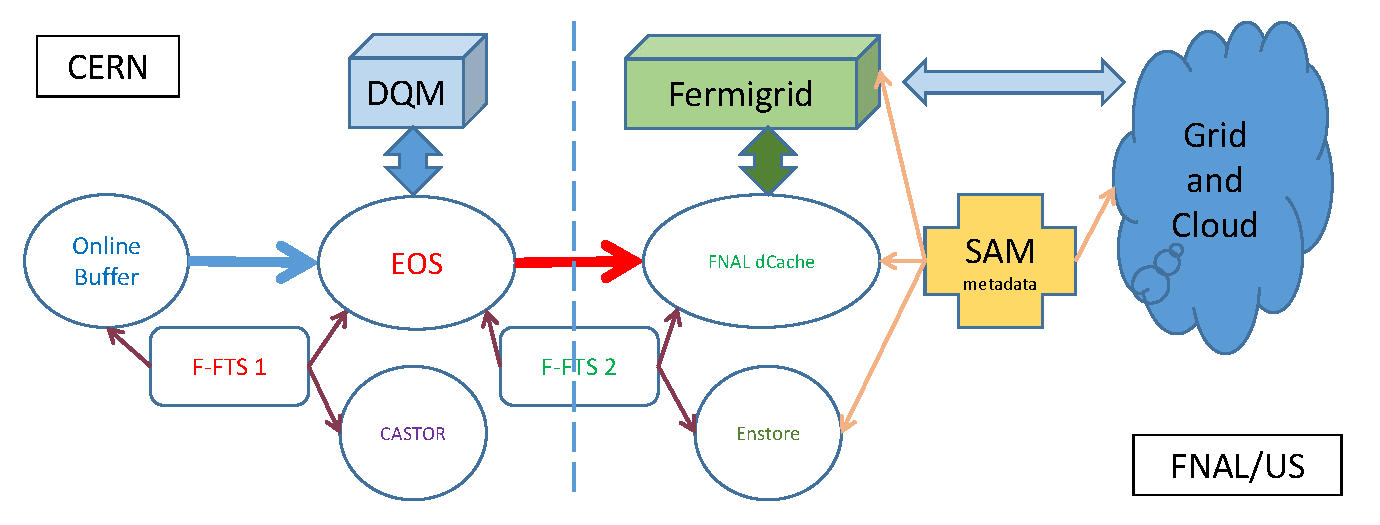
\includegraphics[width=1.0\textwidth]{../figures/data_challenge_1.pdf}
  \caption{Schematics of data flow and  processing in \pd \singp data challenge.}
  \label{fig:dc1}
\end{figure}

\section{Workflows for the Joint Data Challenge - NEEDS Updating}

\subsection{\dualp}

\subsection{\singp}

\begin{itemize}

\item Provide Input Data: 
\begin{itemize}
\item Simulated raw data files will be deposited into an \emph{emulated Online Buffer ( an EOS parition)} by a specially created test agent.
\item A script will be written to deposit or cycle through several files. 
\end{itemize}
\item SAM Metadata is created for the files either by hand or through a script

\item The data  are automatically detected by F-FTS-Lite and transmitted to an EOS dropbox.

\item The input data files are transferred to a few storage locations at Fermilab and CERN and
declared to the file catalog.
\begin{itemize}
\item F-FTS initiates data transfer to dCache and Enstore at FNAL
\item F-FTS initiates data transfer to the input directory of p3s for processing, these directory acts similar to a dropbox and files are then managed by p3s
\item F-FTS initiates data transfer to CASTOR (ongoing discussions of access to tape)
\item Files are updated in SAM
\end{itemize}

\item 

The current proposal is to replicate the BI data to FNAL which would be then the only
source of offline processing including DQM. This may not be ready in time for DC1

\item Automated process initiates DQM streams in p3s which operates using
CERN Tier-0\,\cite{lxbatch}.

\item DQM results (e.g. event display and purity tracker) are provided to users via a dedicated Web service.

\item \textbf{Production team at FNAL submits production jobs using the newly arrived data as input.}
This primarily includes reading the LArTPC data, and the Photon Detector and Beam Instrumentation
systems will be included if ready in time.

\item The Neutrino Platform cluster\,\cite{neut}.

\end{itemize}



\clearpage

\appendix
\section{Files and Interfaces}
\emph{Information here is still under development and subject to discussion. In general it will be pointers to existing documentation  internal to the appropriate components. }
\\ 

%\begin{figure}[tbh]
 % \centering
 % 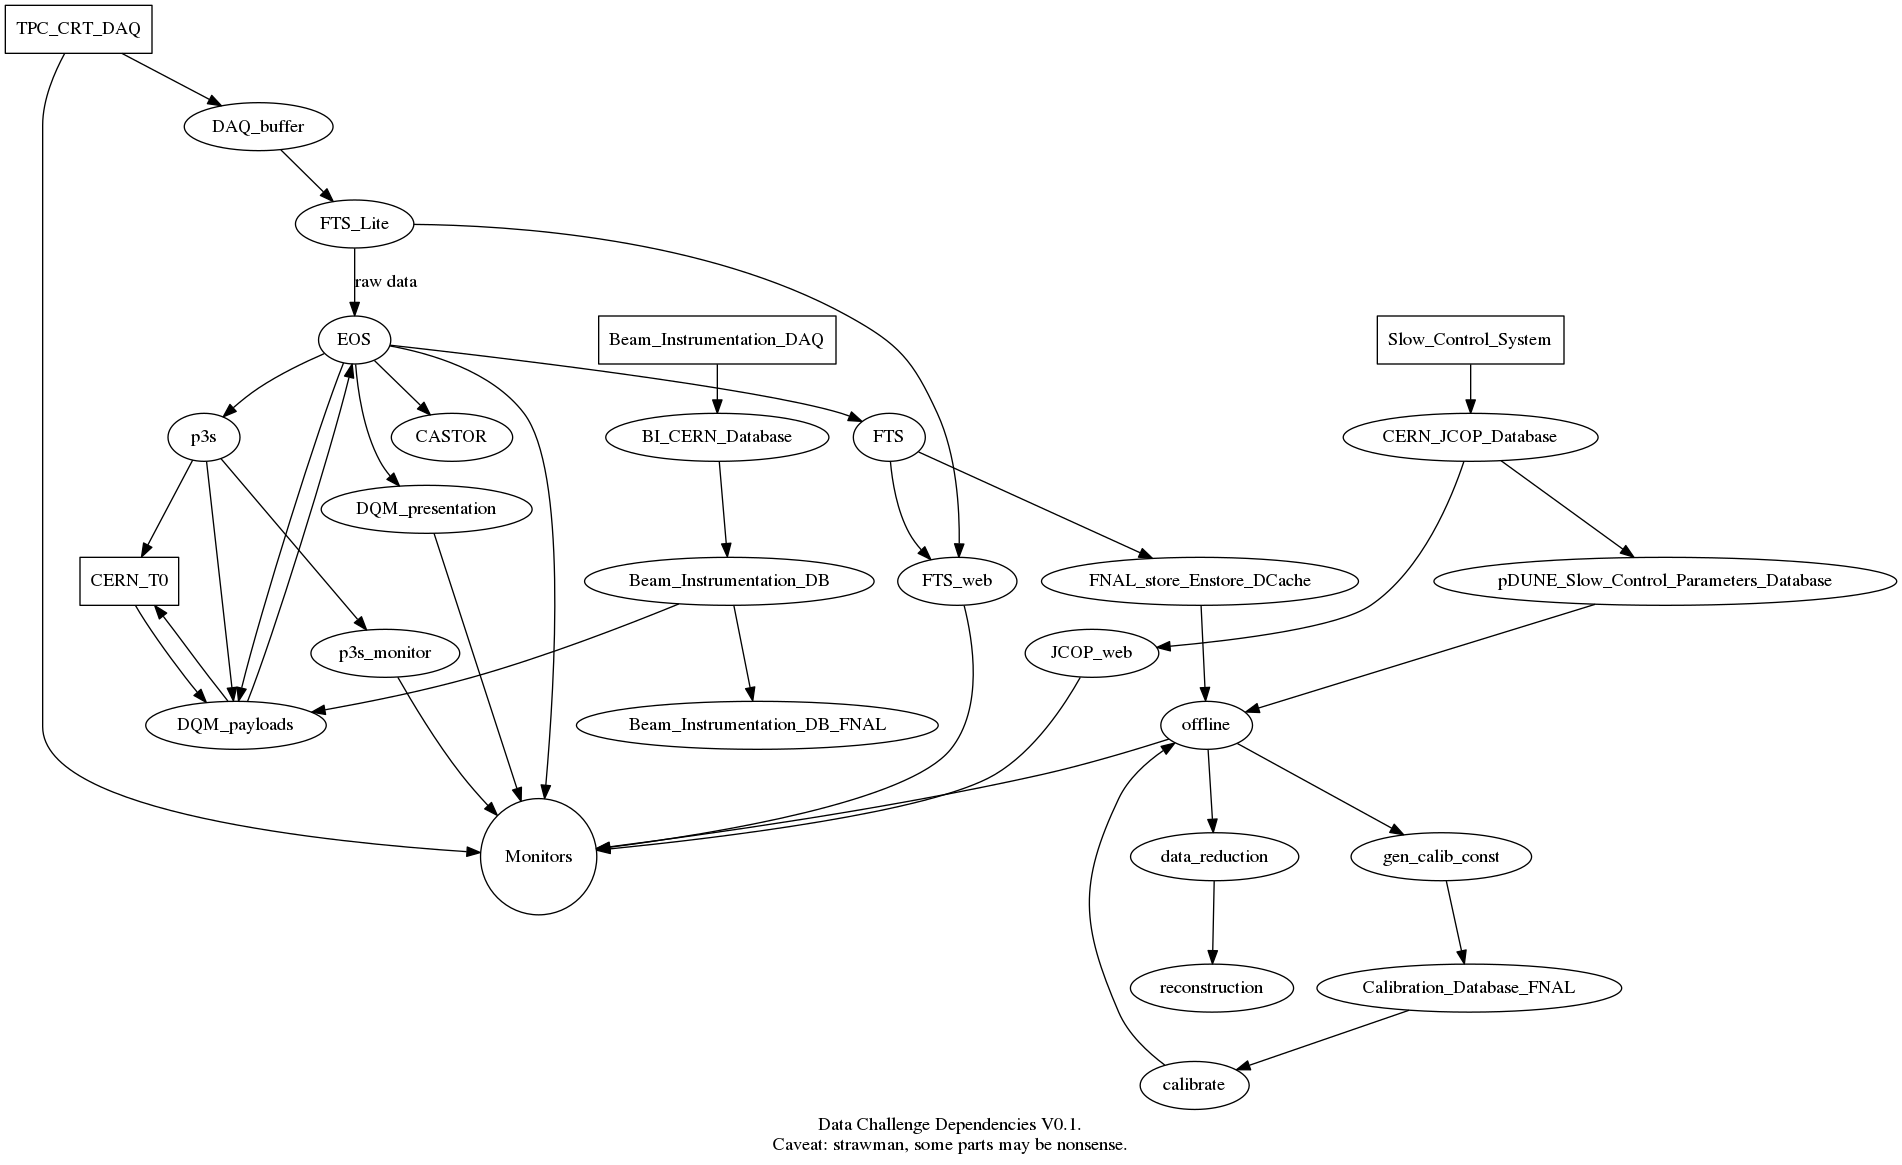
\includegraphics[width=1.0\textwidth]{../figures/dc1_integration.png}
 % \caption{Schematic of Dependencies}
 % \label{fig:dependencies}
%\end{figure}

\renewcommand{\theenumi}{\alph{enumi}}
\begin{enumerate}
\item Beam Instrumentation Database Interface - data format and name of code module and description of the database attributes and internface.
\item Calibration data  -  data format and name of code module and description of the database attributes and interface for calibration information.
\item DQM output files - information about files output from DQM, their location, type and internal format.
\item Input data file - any directory and file naming conventions and details as well as scripts that use this information
\item Input data format - internal format of an input data file
\item POMS configuration files - means of access to and editing of POMS requests.
\item Reduced data format - location of reduced data files (if any) and description of their internal format
\item SAM metadata files  - what SAM metadata files are needed and their description.
\item Slow Control data format - data format and name of code module and description of the database attributes and interface for slow control information.
\end{enumerate}
\renewcommand{\theenumi}{\alph{arabic}}

\noindent Conceptual diagram of the workflows and their dependencies is shown in Figure 2. We aim to make sure that the terminology and its presentation is consistent across components, and comments are welcome.


\begin{thebibliography}{1}

\bibitem{docdb1794}
{DUNE DocDB 1794: \textit{ProtoDUNE-SP Technical Design Report }}\\
\url{http://docs.dunescience.org:8080/cgi-bin/ShowDocument?docid=1794}



\bibitem{docdb1212}
{DUNE DocDB 1212: \textit{Design of the Data Management System for the protoDUNE Experiment}}\\
\url{http://docs.dunescience.org:8080/cgi-bin/ShowDocument?docid=1212}

\bibitem{eos}
{The CERN Exabyte Scale Storage}\\
\url{http://information-technology.web.cern.ch/services/eos-service}


\bibitem{fts}
{The Fermilab File Transfer System}\\
\url{http://cd-docdb.fnal.gov/cgi-bin/RetrieveFile?docid=5412&filename=datamanagement-changeprocedures.pdf&version=1}


\bibitem{docdb1811}
{DUNE DocDB 1811: \textit{Prompt Processing System Requirements for the Single-Phase protoDUNE}}\\
\url{http://docs.dunescience.org:8080/cgi-bin/ShowDocument?docid=1811}

\bibitem{p3s}
{A Design of the Prompt Processing System for the Single-Phase protoDUNE experiment (NP04 )}\\
\url{http://docs.dunescience.org:8080/cgi-bin/ShowDocument?docid=1861}

\bibitem{docdb2089}
{Proposed Initial Data Reduction for protoDUNE/SP}\\
\url{http://docs.dunescience.org/cgi-bin/RetrieveFile?docid=2089}

\bibitem{poms}
{Production Operations Management Service (POMS)}\\
\url{https://cdcvs.fnal.gov/redmine/projects/prod_mgmt_db}


\bibitem{lxbatch}
{The CERN batch computing service}\\
\url{http://information-technology.web.cern.ch/services/batch}



\bibitem{neut}
{Neutrino Computing Cluster at CERN}\\
\url{https://twiki.cern.ch/twiki/bin/view/CENF/NeutrinoClusterCERN}




\end{thebibliography}


\end{document}

%%% Local Variables:
%%% mode: latex
%%% TeX-master: t
%%% End:
\grid
=======
\documentclass[pdftex,12pt,letter]{article}
\usepackage[binary-units=true]{siunitx}
\usepackage[margin=0.75in]{geometry}
\usepackage{verbatim}
\usepackage{graphicx}
\usepackage{cite}
\usepackage{color}
\usepackage[pdftex,pdfpagelabels,bookmarks,hyperindex,hyperfigures]{hyperref}
\usepackage{xspace}
\usepackage{amssymb}


\bibliographystyle{unsrt}

\newcommand{\fixme}[1]{\textbf{FIXME: #1}}    
\newcommand{\pd}{protoDUNE\xspace}

\title{A Proposal for the Single-Phase \pd Experiment Data Challenges in 2017-2018}
\date{\today}
\author{R.Pordes, M.Potekhin, R.Sulej}

\begin{document}


\maketitle

\begin{abstract}



\noindent It is important to ensure 100\% readiness of the
end-to-end \pd software and computing complex during the detector commissioning period and
throughout data taking in 2018. We propose to conduct two Data Challenges (DCs) in order to identify
and address potential issues before they can impact the experiment.
DCs will include defining and  testing interfaces, measuring rates and reliability of data transfers
and job execution, understanding the set of processing workflows, and publishing the results of monitoring
the infrastructure as well as the physics outputs.
Please see the \textit{Revisions} section to learn about evolution of the document.


\end{abstract}

\tableofcontents

\pagebreak

\section{Revisions}
\begin{itemize}

\item Version 1: May 2017 - Initial definition of components of the data challenges

\item Version 2: In progress. Will be used to initially define and agree on the components of DC1. Add some consistent numbering/naming of the steps to be done. Add information on files used/needed.

\end{itemize}

\section{About this document}

The goal of this document is to provide concise information about the proposed \pd Data Challenges
to the individual working groups in order to coordinate effort and come to a consensus as to the scope,
plans and schedule of the proposed Data Challenges. It does not contain detailed descriptions
and/or designs of the \pd computing
infrastructure elements} and the reader is referred to existing documentation where
needed, with references provided in the text.
Information regarding the \pd (NP04) computing is summarized in the \pd-SP Technical Design Report\cite{docdb1794}.

\section{The Scope of the Data Challenges}
\subsection{Assumptions about the software status}
The Data Challenges will be done with the understanding that the software is not in its final state/readiness. 

\subsection{Components}
The following components (including infrastructure, middleware and software) can be identified as relevant in the context
of Data Challenges (which will be also referred to as \textit{``DC''} in this document):
\begin{enumerate}
\item The DAQ \textbf{Online Buffer} which stores raw data assembled by the Event Builders, as files on disk. The internals
of the DAQ system itself are not within the scope.

\item  \textbf{Beam Instrumentation Interface}. Most of the Beam Instrumentation data is not included into the data stream
handled by the \pd DAQ (whose primary task is to capture data from the TPC and the Photon Detector), and is instead
transmitted to the Beam Instrumentation Database at CERN. It is not available immediately for each triggered event,
and is instead available in batches after each spill cycle of the SPS. Interfacing this system is a task that needs
to be addressed for \pd to be able to include these data in its offline processing in an optimal manner.

\item The \textbf{Slow Control and Online Monitoring System} which provide control, monitoring and display of the data acquisition readout and detector parameters. 

\item The \textbf{Data Management System}\cite{docdb1212}  which performs data transfers between a few endpoints
at CERN and FNAL starting with the Online Buffer, including output from DQM,  and which is also tasked with proper accounting and handling of the file catalog and other metadata
by interacting with the SAM system at FNAL (see next item). The Data Management/Handling System will also interface the disk-based mass storage
at CERN and FNAL (i.e.\,EOS\cite{eos} and dCache) as well as tape systems (CASTOR and Enstore respectively).
We anticipate using the \textit{Fermi File Transfer System} (also abbreviated as F-FTS\cite{fts}).

\item The \textbf{File Catalog (Metadata)}  -- SAM system at FNAL which comprises the functionality of the file catalog, data storage and
retrieval based on Metadata and can also be used for orchestration of production workflows.

\item \textbf{Data Quality Monitoring} (DQM) which is tasked with running algorithms with turnaround time short enough to provide
actionable results (under and hour) but which won't fit into the computational footprint of the Online Monitoring (a part of DAQ).
To support DQM, the ProtoDUNE Prompt Processing System (\textbf{p3s}) \cite{docdb1811,p3s} has been created and will run any type of\
DQM workload as formulated and programmed by the working groups.

\item \textbf{Calibration} While it is not expected that these components will be finalized
(and some even exist) at the time of the first Data Challenge it is important to have a firm grasp of the required interfaces,
data flow patterns and other crucial aspects of the \pd Calibration software.
 \item \textbf{Reconstruction}. While it is not expected that these components will be finalized
(and some even exist) at the time of the first Data Challenge it is important to have a firm grasp of the required interfaces,
data flow patterns and other crucial aspects of the \pd Reconstruction Systems. Having prototypes in place is therefore crucial
on the time scale of the Data Challenges.
An important component of the overall production chain is the \textit{Data Reduction} step along the lines described
in \cite{docdb2089}. It combines a few signal-processing procedures (cf. digital filtering and noise reduction), and it will be
necessary in any version or architecture of the production software.
Understanding the interfaces and practical implications of this component would be a useful part of the Data Challenge.

\item \textbf{Analysis Suite Prototypes}. Same comment applies here as to the previous item, i.e.\,while there is no expectation
for the final design and implementation of the analysis chain to exist early in the experiment (especially that it is by nature the most
dynamic and fluid part of all software) it is important to put in place, document and optimize its interfaces with various components
of infrastructure e.g.\,calibration databases, Metadata, software and data provenance controls etc.

\item \textbf{Production Operations Management System (based on POMS)}. This FNAL-based service includes using the DUNE service portal, production workflows executed by POMS \cite{poms}, including the management and automation of  jobs
submission on distributed resources on the Grid. It will be the primary platform for \pd on which to run production and analysis.


\end{enumerate}
\noindent The relationship between the various infrastructure and other components listed above is schematically illustrated in
Fig.\ref{fig:dc1}. This diagram relflects the fact that transmission of \pd data is a multistage process and in particular there
will be separate instances of F-FTS transferring the data from the Online Buffer to mass storage at CERN, and then from
CERN to FNAL and elsewhere.

\begin{figure}[tbh]
  \centering
  \includegraphics[width=1.0\textwidth]{../figures/data_challenge_dp.pdf}
  \caption{Schematics of data flow and  processing for \singp \pd.}
  \label{fig:dc1}
\end{figure}



\begin{figure}[tbh]
  \centering
  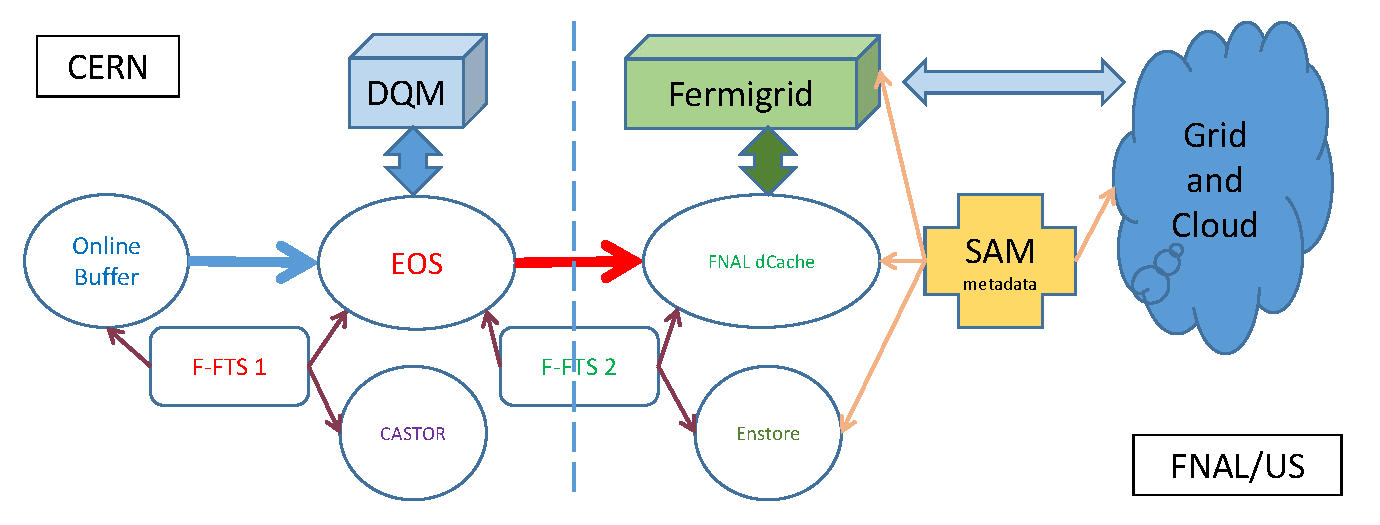
\includegraphics[width=1.0\textwidth]{../figures/data_challenge_1.pdf}
  \caption{Schematics of data flow and  processing for \dualp \pd.}
  \label{fig:dc1}
\end{figure}


\subsection{Files and Interfaces: ** Incomplete/Wrong  - For Discussion **}


The information here will be built up as needed and known. In general it will be pointers to existing documentation  internal to the appropriate components. 
\renewcommand{\theenumi}{\alph{enumi}}
\begin{enumerate}
\item Beam Instrumentation Database Interface - data format and name of code module and description of the database attributes and internface.
\item Calibration data  -  data format and name of code module and description of the database attributes and interface for calibration information.
\item DQM output files - information about files output from DQM, their location, type and internal format.
\item Input data file - any directory and file naming conventions and details as well as scripts that use this information
\item Input data format - internal format of an input data file
\item POMS configuration files - means of access to and editing of POMS requests.
\item Reduced data format - location of reduced data files (if any) and description of their internal format
\item SAM metadata files  - what SAM metadata files are needed and their description.
\item Slow Control data format - data format and name of code module and description of the database attributes and interface for slow control information.
\end{enumerate}
\renewcommand{\theenumi}{\alph{arabic}}

%An ongoing diagram of the workflows and their dependencies is shown in Figure 2: Schematic of Dependencies. It is another %aim of the data challenges to check that terminology, and it's presentation, is consistent across components - work to be done!

%\begin{figure}[tbh]
% \centering
%  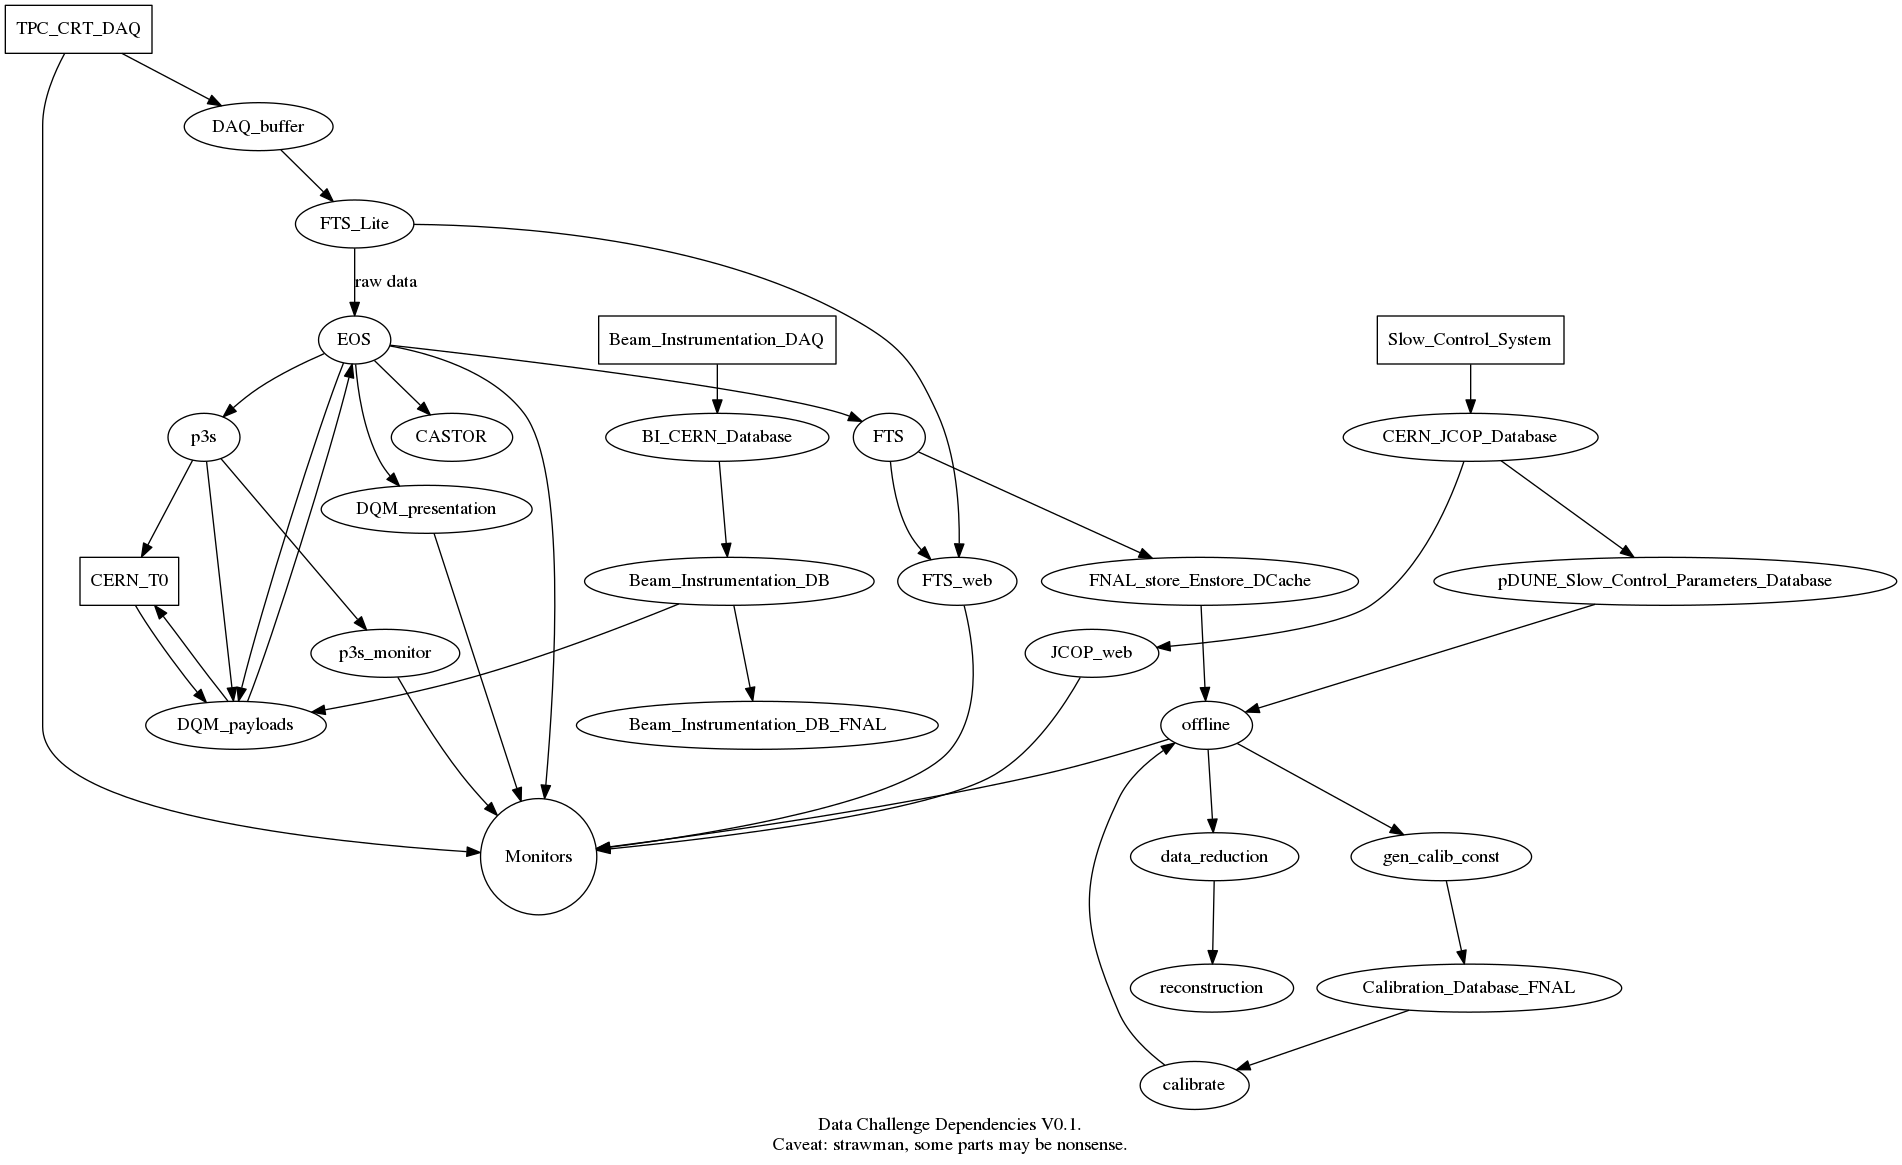
\includegraphics[width=1.0\textwidth]{../figures/dc1_integration.png}
%  \caption{Schematic of Dependencies}
%  \label{fig:dependencies}
%\end{figure}


\section{Data Challenge Process Flow}
\subsection{\dualp}

\section{ \singp}

\begin{itemize}

\item Provide Input Data: 
\begin{itemize}
\item Simulated raw data files will be deposited into a Test/Simulated Online Buffer by a specially created test agent.
\item  Initially this will be on a CERN OpenStack VM for testing of functionality but not performance. 
\item A script will be written to deposit or cycle through several files. 
\end{itemize}
\item SAM Metadata is created for the files either by hand or through a script

\item The data files are automatically detected by F-FTS-Lite and transmitted to EOS.

\item The input data files are transferred to storage at Fermilab and CERN and declared to the file catalog.
\begin{itemize}
\item F-FTS initiates data transfer to dCache and Enstore at FNAL. 
\item F-FTS initiated data transfer to Castor
\item Files are updated in SAM
\end{itemize}

\item  Beam Instrumentation Data

An  instance of the standard IFBeam Database deployed at FNAL for existing Intensity Frontier experiments will be implemented for the protoDUNE-Single Phase Beam Instrumentation database.  A collector process will be running at CERN  reading some device(s) from existing experiment BI databases -  not related to ProtoDUNE.  The Collector produces data files and ingests them into the Fermilab protoDUNE-SP BI database. The latency and throughput of this application will be measured.

In parallel, the offline group is working to populate the  protoDUNE BI DB with simulation generated data. The mock data will then be accessed by an offline algorithm using the standard IFBeam LArSoft API.  If available in time the web interface will be used by the DQM to access this data also. 

\item Automated process initiates DQM streams in p3s which operates using
CERN Tier-0\,\cite{lxbatch}. The Neutrino Platform cluster\,\cite{neut} will not be used at this point.

\item Production team at FNAL submits production jobs using the newly arrived data as input.
This primarily includes reading the LArTPC data, and the Photon Detector and Beam Instrumentation
systems will be included if ready in time.

\end{itemize}



\clearpage


\begin{thebibliography}{1}

\bibitem{docdb1794}
{DUNE DocDB 1794: \textit{ProtoDUNE-SP Technical Design Report }}\\
\url{http://docs.dunescience.org:8080/cgi-bin/ShowDocument?docid=1794}



\bibitem{docdb1212}
{DUNE DocDB 1212: \textit{Design of the Data Management System for the protoDUNE Experiment}}\\
\url{http://docs.dunescience.org:8080/cgi-bin/ShowDocument?docid=1212}

\bibitem{eos}
{The CERN Exabyte Scale Storage}\\
\url{http://information-technology.web.cern.ch/services/eos-service}


\bibitem{fts}
{The Fermilab File Transfer System}\\
\url{http://cd-docdb.fnal.gov/cgi-bin/RetrieveFile?docid=5412&filename=datamanagement-changeprocedures.pdf&version=1}


\bibitem{docdb1811}
{DUNE DocDB 1811: \textit{Prompt Processing System Requirements for the Single-Phase protoDUNE}}\\
\url{http://docs.dunescience.org:8080/cgi-bin/ShowDocument?docid=1811}

\bibitem{p3s}
{A Design of the Prompt Processing System for the Single-Phase protoDUNE experiment (NP04 )}\\
\url{http://docs.dunescience.org:8080/cgi-bin/ShowDocument?docid=1861}

\bibitem{docdb2089}
{Proposed Initial Data Reduction for protoDUNE/SP}\\
\url{http://docs.dunescience.org/cgi-bin/RetrieveFile?docid=2089}

\bibitem{poms}
{Production Operations Management Service (POMS)}\\
\url{https://cdcvs.fnal.gov/redmine/projects/prod_mgmt_db}


\bibitem{lxbatch}
{The CERN batch computing service}\\
\url{http://information-technology.web.cern.ch/services/batch}



\bibitem{neut}
{Neutrino Computing Cluster at CERN}\\
\url{https://twiki.cern.ch/twiki/bin/view/CENF/NeutrinoClusterCERN}




\end{thebibliography}


\end{document}

%%% Local Variables:
%%% mode: latex
%%% TeX-master: t
%%% End:
\grid
>>>>>>> origin/master